\section*{Chương 3: Kết quả và đánh giá}
\addcontentsline{toc}{section}{Chương 3: Kết quả và đánh giá}

\subsection*{1. Phương pháp đánh giá}
\subsubsection*{1.1. Tỷ lệ triệt tiêu dữ liệu (Sparsity)}
\noindent Thông số Sparsity thể hiện tỷ lệ phần tử chi tiết trong ảnh sau khi cắt ngưỡng bị triệt tiêu trên tổng số phần tử của bức ảnh.
$$Sparsity = \frac{N_{zero}}{N_{total}} \times 100\%$$
Trong đó:
\begin{itemize}
    \item $N_{zero}$: Số lượng các phần tử bằng 0 của ảnh sau khi nén.
    \item $N_{total}$: Tổng số lượng điểm ảnh của bức ảnh gốc.
\end{itemize}
\noindent Về mặt ý nghĩa, Sparsity càng cao tức là số lượng phần tử chi tiết bị triệt tiêu trong quá trình nén ảnh càng nhiều,
giúp dung lượng file giảm đi tương đương. Tuy nhiên Sparsity quá cao có thể làm mất chi tiết trong ảnh mặc cho đã tiết kiệm được dung lượng.


\subsubsection*{1.2. Sai số toàn phương trung bình (Mean Squared Eror - MSE)}
\noindent MSE là trung bình bình phương sự chênh lệch từng điểm ảnh giữa ảnh gốc và ảnh đã nén.
$$MSE = \frac{1}{m.n} \sum_{i=1}^{m} \sum_{j=1}^{n} \left[ I(i,j)-K(i,j) \right]^2$$
Trong đó:
\begin{itemize}
    \item $m,n$: Là kích thước của ảnh.
    \item $I$: Ma trận ảnh gốc.
    \item $K$: Ma trận ảnh đã khôi phục.
\end{itemize}
\noindent Nếu $MSE=0$ nghĩa là không có sự chênh lệch nào, ngược lại $MSE$ càng cao càng có sự chênh lệch giữa ảnh gốc và ảnh đã giải nén.


\subsubsection*{1.3. Tỷ số tín hiệu cực đại trên nhiễu (Peak Signal to Noise Ratio - PSNR)}
\noindent Thông số PSNR (đơn vị Decibel - dB) là thông số quan trọng cho biết trực tiếp chất lượng ảnh sau giải nén so với ảnh gốc.
Thông số dựa trên tỉ lệ giữa bình phương phần tử có độ sáng lớn nhất chia cho MSE và được ép tỷ lệ qua hàm logarith.
$$PSNR=10.log_{10} \left( \frac{MAX_I^2}{MSE} \right)$$
Trong đó:
\begin{itemize}
    \item $MAX_I$: Giá trị của điểm ảnh sáng nhất.
    \item $MSE$: Sai số toàn phương trung bình.
\end{itemize}
\noindent PSNR càng cao (lý tưởng từ 30 dB trở lên) tương đương với việc bức ảnh được nén và khôi phục rất tốt, mắt người khó phân biệt
được sự khác biệt với ảnh gốc. Ngược lại PSNR càng thấp, ảnh càng vỡ và mất chi tiết.

\subsubsection*{1.4. Tỷ lệ nén (Compression Ratio)}
Tỷ lệ nén thể hiện tỷ lệ tối ưu về mặt lưu trữ dữ liệu của ảnh nén so với ảnh chưa nén. Ví dụ tỷ lệ nén là $1:4$ tương đương ảnh đã nén chỉ chiếm lượng lưu trữ bằng một phần tư ban đầu.
$$Compression Ratio = \frac{N_{non-zero}}{N_{total}}$$
Trong đó:
\begin{itemize}
    \item $N_{non-zero}$: Số lượng các phần tử khác 0 của ảnh sau khi nén.
    \item $N_{total}$: Tổng số lượng điểm ảnh của bức ảnh gốc.
\end{itemize}

\subsection*{2. Thực hiện đánh giá}
\noindent Thực hiện đánh giá ảnh gốc là ảnh chú chó trong hình sau:
\begin{figure}[H]
    \centering
    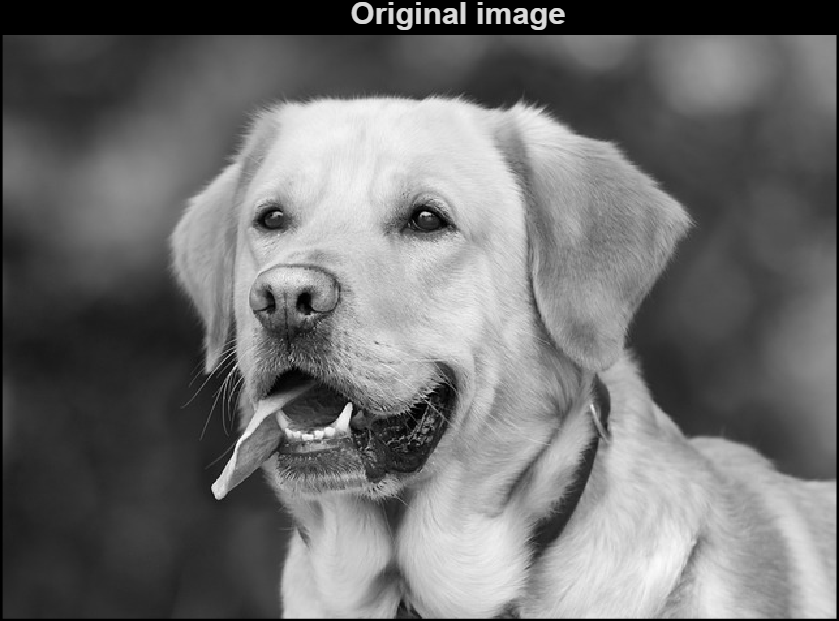
\includegraphics[width=1\textwidth]{dog.png}
    \caption{Ảnh gốc chú chó.}
\end{figure}
\noindent Với các thông số:
\begin{itemize}
    \item $Level=2$.
    \item $Threshold=50$
\end{itemize}

\noindent Thực hiện tái tạo ta thu được ảnh chú chó:
\begin{figure}[H]
    \centering
    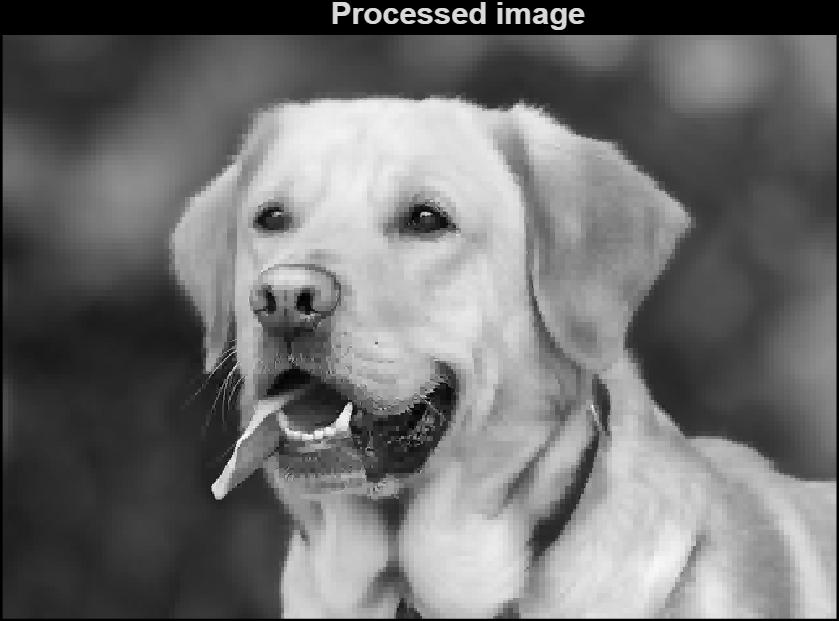
\includegraphics[width=1\textwidth]{Dog_evaluate.png}
    \caption{Ảnh chú chó đã khôi phục.}
\end{figure}
\noindent Kết quả phân tích ảnh thu được như sau:
\begin{itemize}
    \item $MSE=46.12$
    \item $PSNR=31.49 dB$
    \item $Sparsity=93.11\%$
    \item $Compression Ratio = 1:14.50$
\end{itemize}
\noindent Với mức ngưỡng 50 được cho là khá cao, tỷ lệ nén lúc này cho thấy ảnh chú cho khi nén giúp tối ưu lưu trữ đến hơn 14 lần. Để ý ta thấy phần hậu cảnh
được chụp với hiệu ứng bokeh, tức là hậu cảnh đã được làm mờ, tương đương đến sự khác biệt về chi tiết trong hậu cảnh là không đáng kể. Do đó mặc
dù chỉ số PSNR không quá thấp nhưng ta vẫn thấy được sự vỡ ảnh ở chú chó do phần lớn sự triệt tiêu xảy ra trên chú chó này.

\noindent Ở lần thử tiếp theo hãy thử hạ thấp mức ngưỡng xuống còn 20 và xem điều gì sẽ xảy ra:
\begin{figure}[H]
    \centering
    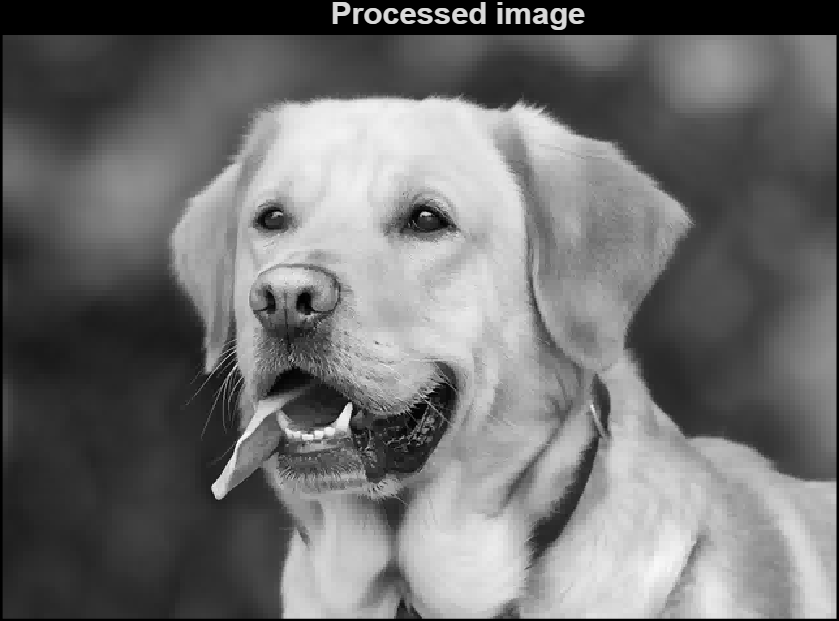
\includegraphics[width=1\textwidth]{Dog_evaluate2.png}
    \caption{Ảnh chú chó đã khôi phục lần thử 2.}
\end{figure}
\noindent Kết quả phân tích ảnh thu được như sau:
\begin{itemize}
    \item $MSE=18.47$
    \item $PSNR=35.47 dB$
    \item $Sparsity=90.15\%$
    \item $Compression Ratio = 1:10.15$
\end{itemize}
\noindent Các chi tiết trên khuôn mặt chú chó lúc này gần như không thể phân biệt so với ảnh gốc, tương ứng với PSNR đã tăng đến 35.47 đánh đổi bằng việc
dung lượng lưu trữ tăng lên nhưng vẫn giữ tỷ lệ đáng kể ít hơn một phần mười so với ảnh gốc.